%%%%%%%%%%%%%%%%%%%%%%%%%%%%%%%%%%%%%%%%%%%%%%%%%%%%%%%%%%%%%%%%%%%%%%%%%%%%%%%%%%%%%%%%%%%%%%%%%%%%%
% The introduction should be succinct, with no subheadings. 
%%%%%%%%%%%%%%%%%%%%%%%%%%%%%%%%%%%%%%%%%%%%%%%%%%%%%%%%%%%%%%%%%%%%%%%%%%%%%%%%%%%%%%%%%%%%%%%%%%%%%

\section{Introduction}

%%%%%%%%%%%%%%%%%%%%%%
% -- Different mechanisms evolve to cope with fluctuating environments, and those mechanisms
%    affect evolution. --
%%%%%%%%%%%%%%%%%%%%%%
%Fluctuating environmental conditions are ubiquitous in natural systems. 
Natural organisms employ a wide range of evolved strategies for coping with environmental change, such as 
periodic migration \citep{winger_long_2019}, 
bet-hedging \citep{beaumont_experimental_2009}, 
adaptive tracking \citep{barrett_adaptation_2008}
and phenotypic plasticity \citep{ghalambor_adaptive_2007}.
The particular mechanisms that evolve in response to fluctuating environments will also shift the course of subsequent evolution \citep{wennersten_population-level_2012,schaum_plasticity_2014}.
%Identifying the mechanisms most likely to evolve and examining both the evolutionary constraints and opportunities associated with each is critical for us to understand and predict evolutionary outcomes in changing environments.
As such, if we are to understand or predict evolutionary outcomes we must be able to identify which mechanisms are most likely to evolve and what constraints and opportunities they impart on subsequent evolution.

%%%%%%%%%%%%%%%%%%%%%%
% -- We focus on how plasticity affects subsequent evolution. --
%%%%%%%%%%%%%%%%%%%%%%
In this work, we focus on phenotypic plasticity, which can be defined as the capacity for a single genotype to alter phenotypic expression in response to a change in its environment \citep{west-eberhard_developmental_2003}. 
Phenotypic plasticity is controlled by genes whose expression is coupled to one or more environmental signals, which may be either biotic or abiotic. 
For example, the sex ratio of the crustacean \textit{Gammarus duebeni} is modulated by changes in photoperiod and temperature \citep{dunn_two_2005}, and the reproductive output of some invertebrate species is heightened when infected with parasites to compensate for offspring loss \citep{chadwick_parasite-mediated_2005}. 
In this study, we conducted digital evolution experiments to investigate how the evolution of adaptive phenotypic plasticity shifts the course of evolution in a cyclically changing environment.
Specifically, we examined the effects of adaptive plasticity on subsequent genomic and phenotypic change, the capacity to evolve and then maintain novel traits, and the accumulation of deleterious alleles.


%%%%%%%%%%%%%%
% Effects of phenotypic plasticity on subsequent evolution disputed.
%   - baseline expections on rate of evolutionary response given adaptive vs. non-adaptive plasticity
%%%%%%%%%%%%%%
Evolutionary biologists have long been interested in how evolutionary change is influenced by phenotypic plasticity because of its role in generating phenotypic variance \citep{gibert_phenotypic_2019}.
The effects of phenotypic plasticity on adaptive evolution have been disputed, as few studies have been able to observe both the initial patterns of plasticity and the subsequent divergence of traits in natural populations \citep{ghalambor_adaptive_2007,wund_assessing_2012,forsman_rethinking_2015,ghalambor_non-adaptive_2015,hendry_key_2016}.
In changing environments, adaptive phenotypic plasticity provides a mechanism for organisms to regulate trait expression within their lifetime, which can stabilize populations through those changes \citep{gibert_phenotypic_2019}.
In this context, the stabilizing effect of adaptive plasticity has been hypothesized to constrain the rate of adaptive evolution \citep{gupta_study_1982,ancel_undermining_2000,huey_behavioral_2003,price_role_2003,paenke_influence_2007}.
That is, directional selection may be weak if environmentally-induced phenotypes are close to the optimum; as such, adaptively plastic populations may evolve slowly (relative to non-plastic populations) unless there is a substantial fitness cost to plasticity.

% @AML: Caption needs some streamlining/work!
\begin{figure}[h!]
    \centering
    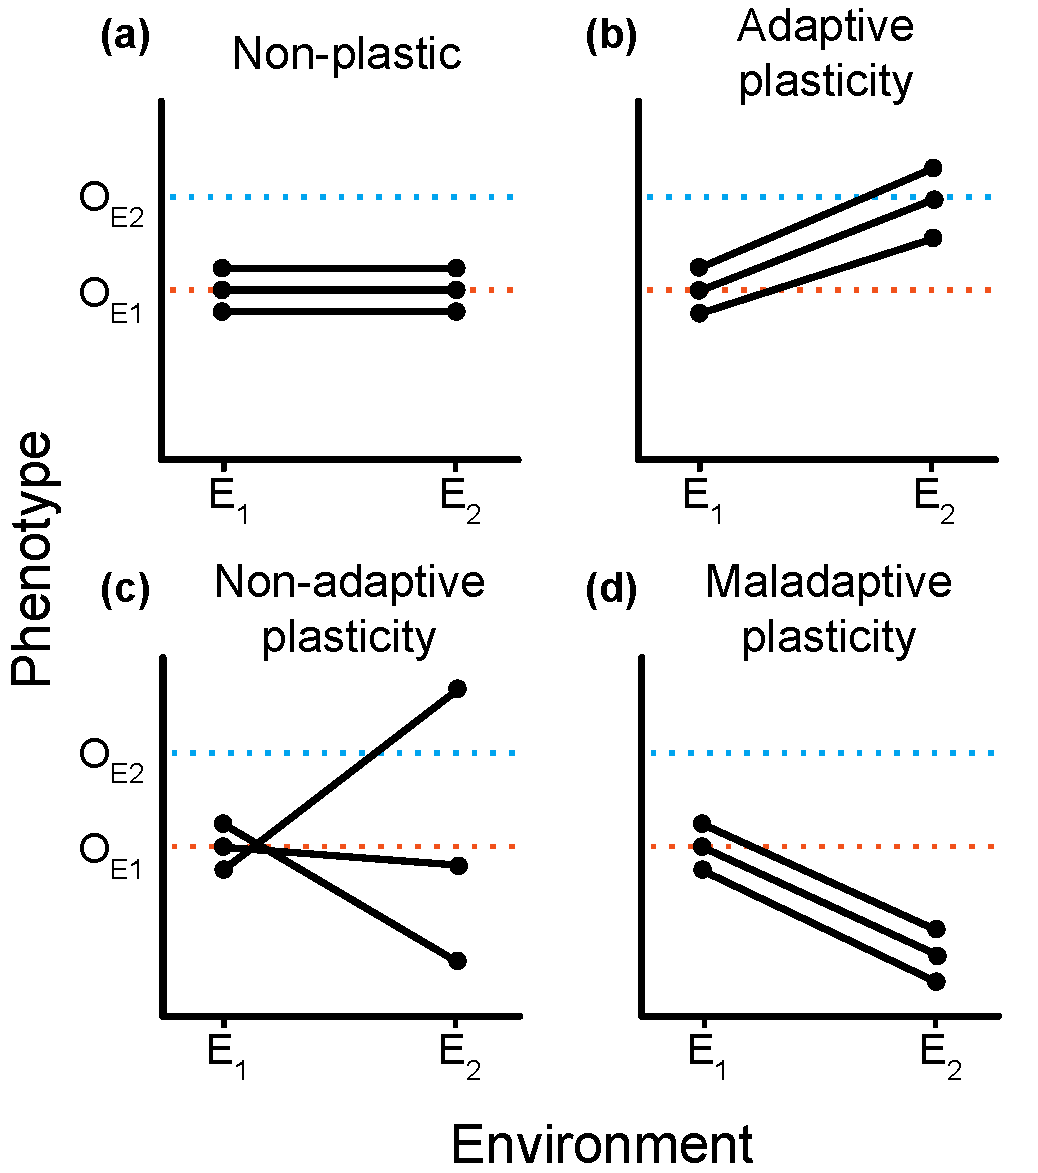
\includegraphics[width=\textwidth]{media/reaction-norms.pdf}
    \caption{\small
    \textbf{todo.}
    todo.
    }
    \label{fig:reaction-norms}
\end{figure}

% Feedback
%  - Ideas: color background red/blue
%  - Titles on (a), (b), (c), (d)?
%    - Swap (c) & (d)
%    - non-plastic, adaptive plasticity, non-adaptive plasticity, maladaptive plasticity
%  - (e) environmental scenario/environment
% - Increase font sizes
% - pull word that says time outside the arrow, make arrow smaller, make environment bar bigger => increase font size

% -- Plasticity as a source of cryptic variation --
Phenotypic plasticity allows for the accumulation of genetic variation in genomic regions that are unexpressed under current environmental conditions.
Such cryptic (``hidden'') genetic variation can serve as a source of diversity in the population, upon which selection can act when the environment changes \citep{schlichting_hidden_2008,levis_evaluating_2016}.  
It remains unclear to what extent and under what circumstances this cryptic variation caches adaptive potential or merely accumulates deleterious alleles \citep{gibson_uncovering_2004,paaby_cryptic_2014,zheng_cryptic_2019}.

% -- Genes as followers --
The ``genes as followers'' hypothesis (also known as the ``plasticity first'' hypothesis) predicts that phenotypic plasticity may facilitate adaptive evolutionary change by producing variants with enhanced fitness under stressful or novel conditions \citep{west-eberhard_developmental_2003,schwander_genes_2011,levis_evaluating_2016}. 
Environmentally-induced trait changes can be refined through selection over time (\textit{i.e.}, genetic accommodation).
Further, selection may drive plastic phenotypes to lose their environmental dependence over time in a process known as genetic assimilation \citep{west-eberhard_developmental_2005,pigliucci_phenotypic_2006,crispo_baldwin_2007,schlichting_phenotypic_2014,levis_evaluating_2016}. 
In this way, environmentally-induced phenotypic changes can precede an evolutionary response.

% -- Plastic rescue + wrap up on plasticity background? --
Phenotypic plasticity may also ``rescue'' populations from extinction under changing environmental conditions by buffering populations against novel stressors.
This buffer promotes stability and persistence and grants populations time to further adapt to rapidly changing environmental conditions \citep{west-eberhard_developmental_2003,chevin_when_2010}. 

Disparate predictions about how phenotypic plasticity may shift the course of subsequent evolution are not necessarily mutually exclusive.
Genetic and environmental contexts determine if, and to what extent, phenotypic plasticity promotes or constrains subsequent evolution.
Figure \ref{fig:reaction-norms} overviews how we might expect different forms of phenotypic plasticity to result in different evolutionary responses after an environmental change.

%%%%%%%%%%%%%%%%%%%%%%
% -- Digital evolution --
%%%%%%%%%%%%%%%%%%%%%%
Experimental studies investigating the relationship between phenotypic plasticity and evolutionary outcomes can be challenging to conduct in natural systems.
Such experiments would require the ability to irreversibly toggle plasticity followed by long periods of evolution during which detailed phenotypic data would need to be collected.
Digital evolution experiments have emerged as a powerful research framework from which evolution can be studied.
In digital evolution, self-replicating computer programs (digital organisms) compete for resources, mutate, and evolve following Darwinian dynamics  \citep{wilke_biology_2002}.
Digital evolution studies balance the speed and transparency of mathematical and computational simulations with the open-ended realism of laboratory experiments.
Modern computers allow us to observe many generations of digital evolution at tractable time scales; thousands of generations can take mere minutes as opposed to months, years, or centuries.
Digital evolution systems also allow for perfect, non-invasive data tracking.
Such transparency permits the tracking of complete evolutionary histories within an experiment, which circumvents the historical problem of drawing evolutionary inferences using incomplete records (from frozen samples or fossils) and extant genetic sequences.
Additionally, digital evolution systems allow for experimental manipulations and analyses that go beyond what is possible in wet-lab experiments.
Such analyses have included exhaustive knockouts of every site in a genome to identify the functionality of each \citep{lenski_evolutionary_2003},
comprehensive characterization of local mutational landscapes \citep{lenski_genome_1999,canino-koning_fluctuating_2019},
and the real-time reversion of all deleterious mutations as they occur to isolate their long-term effects on evolutionary outcomes \citep{covert_experiments_2013}. 
Furthermore, digital evolution studies allow us to directly toggle the possibility for adaptive plastic responses to evolve, which enables us to empirically test hypotheses that were previously relegated to theoretical analyses.

%%%%%%%%%%%%%%%%%%%%%%
% -- Overview of what we're testing / doing --
%%%%%%%%%%%%%%%%%%%%%%
In this work, we use the Avida Digital Evolution Platform \citep{ofria_avida:_2009}.
Avida is an open-source system that has been used to conduct a wide range of well-regarded studies on evolutionary dynamics, including 
the origins of complex features \citep{lenski_evolutionary_2003},
the survival of the flattest effect \citep{wilke_evolution_2001},
and the origins of reproductive division of labor \citep{goldsby_evolutionary_2014}.
% @AML: next bit is a little awkward
Our experiments build directly on previous studies in Avida that characterized the \textit{de novo} evolution of adaptive phenotypic plasticity \citep{clune_investigating_2007,lalejini_evolutionary_2016} as well as previous work investigating the evolutionary consequences of fluctuating environments for populations of non-plastic digital organisms \citep{li_digital_2004,canino-koning_fluctuating_2019}.
Of particular relevance, \cite{clune_investigating_2007} and \cite{lalejini_evolutionary_2016} experimentally demonstrated that adaptive phenotypic plasticity can evolve given the following four conditions (as identified by \citealt{ghalambor_behavior_2010}):
(1) populations experience temporal environmental variation,
(2) these environments are differentiable by reliable cues,
(3) each environment favors different phenotypic traits,
and (4) no single phenotype exhibits high fitness across all environments.
We build on this previous work, but we shift our focus from the evolutionary causes of adaptive phenotypic plasticity to investigate its evolutionary consequences in a fluctuating environment.

%%%%%%%%%%%%%%%%%

% - what we did -
Each of our experiments are divided into two phases: in phase one, we precondition sets of founder organisms with differing plastic or non-plastic adaptations;
in phase two, we examine the subsequent evolution of populations founded with organisms from phase one under specific environmental conditions (Figure \ref{fig:experimental-design}).
First, we examine the evolutionary histories of phase two populations to test whether adaptive plasticity constrained subsequent genomic and phenotypic changes. 
Next, we evaluate how adaptive plasticity influences exploration and exploitation by identifying how well populations produced by each type of founder can evolve and retain novel adaptive traits.
Finally, we examine lineages to determine whether adaptive plasticity facilitated the accumulation of cryptic genetic variation that would prove deleterious when the environment changed. 

%%%%%%%%%%%%%%%%%%%%%%
% - Overview of findings -
%%%%%%%%%%%%%%%%%%%%%%
We found that the evolution of adaptive plasticity reduced subsequent rates of evolutionary change in a cyclic environment.
The non-plastic populations underwent more frequent selective sweeps and accumulated many more genetic changes over time, as non-plastic populations relied on genetic variation from \textit{de novo} mutations to continuously re-adapt to environmental changes. 
The evolution of adaptive phenotypic plasticity buffered populations against environmental fluctuations, whereas repeated selective sweeps in non-plastic populations drove the accumulation of deleterious mutations and the loss of secondary beneficial traits via deleterious hitchhiking.
As such, adaptively plastic populations were better able to retain novel traits than their non-plastic counterparts.
In general, the evolution of adaptive phenotypic plasticity shifted evolutionary dynamics to be more similar to that of populations evolving in a static environment than to non-plastic populations evolving in an identical fluctuating environment. 

% We additionally found no evidence of delthat the evolution of adaptive phenotypic plasticity 
% In addition, we did not find evidence that the evolution of adaptive plasticity resulted in increased rates of deleterious mutation accumulation. 
